\section{Deterministische Modellen}

Als het op het optimaliseren van de voorraad aankomt zijn er \textit{twee kernvragen}:
\begin{enumerate}
    \item Wanneer ga ik een bestelling plaatsen om de vooraad terug aan te vullen? ($OP$)
    \item Hoeveel ga ik bestellen? ($Q$)
\end{enumerate}

Een deterministisch model zal deze vragen trachten te beantwoorden onder de assumptie dat de vraag~($D$) constant is. De vraag is dus gekend en daarenboven ook elke dag hetzelfde.

Het doel is dus de minimalisatie van de kosten. Zo zijn er vier:
\begin{itemize}
    \item Aankoopkosten ($C_p$): aankoopprijs per gekochte eenheid.
    \item Bestel-/omstelkosten ($C_o$): kosten voor transport, omstellen van machines, etc. Vaak onafhankelijk van $Q$.
    \item Tekortkosten ($C_s$): kost per eenheid tekort
    \item Voorraadkosten ($C_h$): ``holding cost'', de kosten om voorraad aan te houden, ook de kapitaalkost ervan. Vaak uitgedrukt als percentage van de aankoopprijs: $C_h = i C_p$
\end{itemize}

\begin{figure}[htbp]
    \centering
    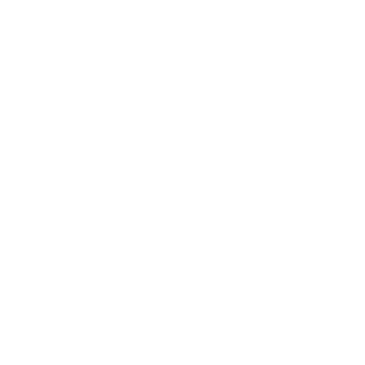
\includegraphics[scale=0.4]{Images/white.png}
    \caption{Het zaagtandmodel (fig 11 boek)}
    \label{fig:zaagtandmodel}
\end{figure}
In figuur~\ref{fig:zaagtandmodel} kan je het typische voorraadverloop zien, waarbij er een $Q$ geleverd wordt, en de voorraad daarna terug afneemt met een snelheid $D$. Vlak voor we uit voorraad zijn bestellen we terug zodat we nooit zonder voorraad zitten.

Wanneer bestellen we dan? Veronderstel de gegevens op slide 2a:3. Werken in twee stappen:
\begin{enumerate}
    \item Eerst berekenen we het order punt ($OP$). We moeten 2 weken levertermijn ($L$) kunnen overbruggen dus we vinden het volgende:
    \begin{equation*}
        OP = 2 \text{ weken } \times \frac{10000\text{/jaar}}{52} = 384
    \end{equation*}
    Wanneer de voorraad dus 384 bedraagt zullen we onze bestelling plaatsen

    \item Vervolgens berekenen we hoeveel we moeten bestellen ($Q$). Om $Q$ te vinden zoeken we het punt waarmee we de kosten op jaarbasis minimaliseren. Deze kosten worden grafisch voorgesteld in figuur~\ref{fig:kostenGrafisch}.
    \begin{figure}[htbp]
        \centering
        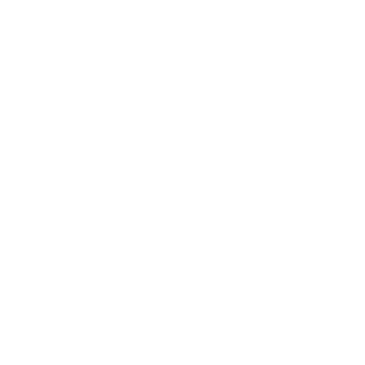
\includegraphics[scale=0.4]{Images/white.png}
        \caption{Grafische voorstelling van de kostenfuncties (fig 12 boek)}
        \label{fig:kostenGrafisch}
    \end{figure}

    We bekomen volgende vergelijking voor de kosten op jaarbasis:
    \begin{equation}
        TK(Q) = D \times C_p + C_o \times \frac{D}{Q} + C_h \times \frac{Q}{2} \label{eq:jaarlijkseKosten}
    \end{equation}
    Als we het minimum van deze functie zoeken bekomen we dat:
    \begin{equation}
        \frac{dTK(Q)}{dQ} \Rightarrow Q = \sqrt{\frac{2 \times D \times C_o}{C_h}} = EOQ \label{eq:eoq}
    \end{equation}
    waarbij $EOQ$ staat voor Economic Order Quantity. We kunnen de getallen voor deze $EOQ$ gewoon invullen en dan bekomen we de optimale $Q$, ook genoteerd als $Q^*$.

\end{enumerate}

\subsection{Inzichten uit de EOQ}
We kunnen formule~\ref{eq:eoq} invullen in formule~\ref{eq:jaarlijkseKosten} om zo de jaarlijkse kosten meteen uit te kunnen rekenen.

Anderzijds kunnen we de Optimale Cyclische Voorraad berekenen. Dit is de voorraad die je aanhoudt ten gevolge van $Q^*$:
\begin{equation}
    \frac{Q}{2} = \frac{\sqrt{\frac{2 \times D \times C_o}{C_h}}}{2} = \sqrt{\frac{D \times C_o}{2 \times C_h}}
\end{equation}

Daarnaast kunnen we ook het aantal bestellingen in het optimum ($N^*$) berekenen:
\begin{equation}
    N^* = \frac{D}{Q} = \frac{D}{\sqrt{\frac{2 \times D \times C_o}{C_h}}} = \sqrt{\frac{D \times C_h}{2 \times C_o}}
\end{equation}

Analoog kan je ook nog de optimale tijd tussen twee bestellingen ($T^* = 1 / N^*$) berekenen.

\subsection{Centraal vs. Decentraal}
Er zijn twee manieren om je logistieke keten op te zetten: de centrale- en decentrale manier. Bij een decentraal systeem zit je dicht bij de markt, maar een centraal systeem zal in de vraag van alle regios voorzien. Stel dat je $n$ distributiecentra hebt, dan zou een systeem met een centraal magazijn toelaten om je voorraad met een factor $\sqrt{n}$ te verminderen. (zie berekening in nota's)

Deze opmerking is gelijk aan de volgende: indien de vraag stijgt met $n$, zal de voorraad slechts met $\sqrt{n}$ toenemen.

\subsection{Deterministisch model voor meerdere producten}
Wat als ons bedrijf meerdere producten verkoopt? $\Rightarrow C_o$ heeft een vaste component plus een variabele component per product. We zouden de bestelcyclus voor elk product apart kunnen optimaliseren, maar dan kan het voorvallen dat we soms bestelling vlak na elkaar ontvangen. Oplossing: alles samen bestellen en dus $N$ optimaliseren in plaats van $Q$.

Dit doen we als volgt:
\begin{equation}
    N = \sqrt{\frac{D \times C_h}{2 \times C_o}} = \sqrt{\frac{D \times (C_p \times i)}{2 \times C_o}}
\end{equation}
Merk op dat $D \times C_p$ gelijk is aan het aankoopbedrag op jaarbasis ($D^\$$). Hoeveel bestellen we dan voor elk product $i$?
\begin{equation}
    Q_i^* = \frac{D_i}{N^*}
\end{equation}


\subsection{Productiemodel}
Tot nu toe krijgen we de ganse $Q$ in \'e\'en keer als een levering, maar voor productieomgevingen kan het zijn dat je elke geproduceerde eenheid meteen als voorraad beschikbaar hebt (= \textbf{model met eindige opvulsnelheid}).

\begin{figure}[htbp]
    \centering
    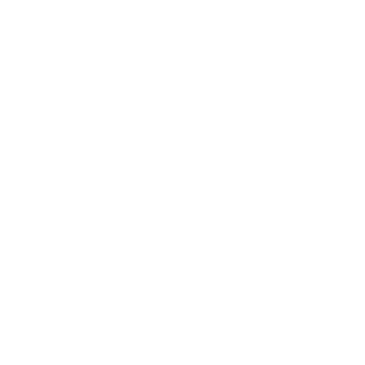
\includegraphics[scale=0.4]{Images/white.png}
    \caption{Het productiemodel (fig 21 boek)}
    \label{fig:productiemodel}
\end{figure}
Zoals je kan zien in figuur~\ref{fig:productiemodel} volgt het voorraadverloop niet meer het klassieke zaagtandmodel omdat de voorraad slechts geleidelijk wordt aangevuld (zie nota's voor extra aantekeningen bij grafiek).

Wederom stellen we ons de vraag wanneer we gaan bijproduceren, en hoeveel dat dan juist moet zijn. Dit noemen we nu niet meer de $EOQ$, maar de $EPQ$. De totale kosten bij een productiemodel zijn als volgt:

\begin{equation}
    TK = D \times C_p + \frac{D}{Q} \times C_o + \frac{Q}{2} \left( 1 - \frac{P}{D} \right) \times C_h
\end{equation}

Als we aan de hand van deze vergelijking de $EPQ$ zoeken krijgen we het volgende:

\begin{equation}
    EPQ = \sqrt{\frac{2 \times D \times C_o}{C_h} \times \frac{1}{ ( 1 - D/P )} }
\end{equation}


\subsection{Hoeveelheidskorting}
Tot nu toe was de aankoopprijs altijd constant, maar wat bij hoeveelheidskortingen? Zoals je kan zien in figuur~\ref{fig:hoeveelheidskortingen}, is de TC-curve niet meer constant doordat de aankoopkost niet meer constant is. Deze heeft nu een trapvormig verloop gekregen. Bijgevolg kunnen we deze niet meer afleiden om zo het optimum te vinden.
\begin{figure}[htbp]
    \centering
    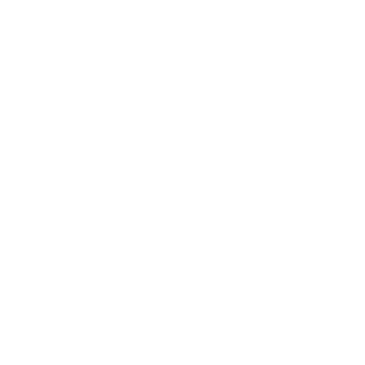
\includegraphics[scale=0.4]{Images/white.png}
    \caption{Het model met hoeveelheidskortingen (fig 16 boek)}
    \label{fig:hoeveelheidskortingen}
\end{figure}

Er is daarom een \textit{algoritme} dat je kan gebruiken om $Q^*$ te vinden. Dit werkt op volgende manier:
\begin{enumerate}
    \item Bereken EOQ voor de laagste aankoopprijs. Indien je deze $Q$ zou kunnen kopen voor die prijs heb je het optimum gevonden. Indien $Q$ te laag is ga je naar de volgende stap.
    \item Indien $Q$ te laag is, wil dat zeggen dat de best mogelijke bestelhoeveelheid voor die prijs, het minimum voor die prijs is. Bereken dus de $TC$ voor die $Q$.
    \item Neem de eerst volgende hogere aankoopprijs en bereken de $EOQ$. Indien deze geldig is voor dat segment vergelijk je de $TC$ onder die $EOQ$ met de eerder gevonden $TC$ van de vorige, lagere prijs.

    Indien ook deze $EOQ$ ongeldig is, bereken je wederom de $TC$ voor de laagste $Q$ in deze categorie en herhaal je het proces voor de volgende, hogere prijs.
\end{enumerate}
